%% This is file `elsarticle-template-5-harv.tex',
%%
%% Copyright 2009 Elsevier Ltd
%%
%% This file is part of the 'Elsarticle Bundle'.
%% ---------------------------------------------
%%
%% It may be distributed under the conditions of the LaTeX Project Public
%% License, either version 1.2 of this license or (at your option) any
%% later version.  The latest version of this license is in
%%    http://www.latex-project.org/lppl.txt
%% and version 1.2 or later is part of all distributions of LaTeX
%% version 1999/12/01 or later.
%%
%% The list of all files belonging to the 'Elsarticle Bundle' is
%% given in the file `manifest.txt'.
%%
%% Template article for Elsevier's document class `elsarticle'
%% with harvard style bibliographic references
%%
%% $Id: elsarticle-template-5-harv.tex 159 2009-10-08 06:08:33Z rishi $
%% $URL: http://lenova.river-valley.com/svn/elsbst/trunk/elsarticle-template-5-harv.tex $
%%
\documentclass[preprint,authoryear,12pt]{elsarticle}

%% Use the option review to obtain double line spacing
%% \documentclass[authoryear,preprint,review,12pt]{elsarticle}

%% Use the options 1p,twocolumn; 3p; 3p,twocolumn; 5p; or 5p,twocolumn
%% for a journal layout:
%% \documentclass[final,authoryear,1p,times]{elsarticle}
%% \documentclass[final,authoryear,1p,times,twocolumn]{elsarticle}
%% \documentclass[final,authoryear,3p,times]{elsarticle}
%% \documentclass[final,authoryear,3p,times,twocolumn]{elsarticle}
%% \documentclass[final,authoryear,5p,times]{elsarticle}
%% \documentclass[final,authoryear,5p,times,twocolumn]{elsarticle}

%% if you use PostScript figures in your article
%% use the graphics package for simple commands
%% \usepackage{graphics}
%% or use the graphicx package for more complicated commands
%% \usepackage{graphicx}
%% or use the epsfig package if you prefer to use the old commands
%% \usepackage{epsfig}

%% The amssymb package provides various useful mathematical symbols
\usepackage{amssymb}
%% The amsthm package provides extended theorem environments
%% \usepackage{amsthm}
\usepackage{color}
\usepackage{siunitx}

%% The lineno packages adds line numbers. Start line numbering with
%% \begin{linenumbers}, end it with \end{linenumbers}. Or switch it on
%% for the whole article with \linenumbers after \end{frontmatter}.
%% \usepackage{lineno}

%% natbib.sty is loaded by default. However, natbib options can be
%% provided with \biboptions{...} command. Following options are
%% valid:

%%   round  -  round parentheses are used (default)
%%   square -  square brackets are used   [option]
%%   curly  -  curly braces are used      {option}
%%   angle  -  angle brackets are used    <option>
%%   semicolon  -  multiple citations separated by semi-colon (default)
%%   colon  - same as semicolon, an earlier confusion
%%   comma  -  separated by comma
%%   authoryear - selects author-year citations (default)
%%   numbers-  selects numerical citations
%%   super  -  numerical citations as superscripts
%%   sort   -  sorts multiple citations according to order in ref. list
%%   sort&compress   -  like sort, but also compresses numerical citations
%%   compress - compresses without sorting
%%   longnamesfirst  -  makes first citation full author list
%%
%% \biboptions{longnamesfirst,comma}

% \biboptions{}

\journal{Biosystems Engineering}

\begin{document}

\begin{frontmatter}

%% Title, authors and addresses

%% use the tnoteref command within \title for footnotes;
%% use the tnotetext command for the associated footnote;
%% use the fnref command within \author or \address for footnotes;
%% use the fntext command for the associated footnote;
%% use the corref command within \author for corresponding author footnotes;
%% use the cortext command for the associated footnote;
%% use the ead command for the email address,
%% and the form \ead[url] for the home page:
%%
%% \title{Title\tnoteref{label1}}
%% \tnotetext[label1]{}
%% \author{Name\corref{cor1}\fnref{label2}}
%% \ead{email address}
%% \ead[url]{home page}
%% \fntext[label2]{}
%% \cortext[cor1]{}
%% \address{Address\fnref{label3}}
%% \fntext[label3]{}

% \title{An Autonomous Platform for Use in Kiwifruit Orchards}
\title{A Platform for Autonomous Navigation in Kiwifruit Orchards}

%% use optional labels to link authors explicitly to addresses:
%% \author[label1,label2]{<author name>}
%% \address[label1]{<address>}
%% \address[label2]{<address>}

% \author{Mark H. Jones, Jamie Bell, Matthew Seabright, Joshua Barnett, Alistair Scarfe, Bruce MacDonald, Mike Duke}

%% Group authors per affiliation:
\author[UoW]{Mark H. Jones\corref{mjemail}} 
\cortext[mjemail]{markj@waikato.ac.nz}

\author[UoA]{Jamie Bell\corref{jbemail}}
\cortext[jbemail]{jamie977@gmail.com}
\author[UoW]{Matthew Seabright}
\author[UoW]{Josh Barnett}
\author[RPL]{Alistair Scarfe}
\author[UoW]{Mike Duke}
\author[UoA]{Bruce MacDonald}

\address[UoW]{School of Engineering, University of Waikato, Hamilton, New Zealand}
\address[UoA]{Faculty of Engineering, University of Auckland, Auckland, New Zealand}
\address[RPL]{Robotics Plus Ltd, Newnham Innovation Park, Tauranga, New Zealand}

\begin{abstract}
%% Text of abstract

    This will be written last.
    General tone of paper is:
    We present a vehicle designed specifically for autonomous control in kiwifruit orchards.
    Here are some other people who have made autonomous specific vehicles.
    Here is ours and this is how it fits in with those.
    We've gone with these sensors and this method of navigation and it has demonstrated itself to work in the orchard.
    We think that we could improve the thing by using this algorithm and increasing module space.
    Generally it is an improvement on the previous work of Scarfe.
\end{abstract}

\begin{keyword}
%% keywords here, in the form: keyword \sep keyword

%% MSC codes here, in the form: \MSC code \sep code
%% or \MSC[2008] code \sep code (2000 is the default)

\end{keyword}

\end{frontmatter}

% \linenumbers

%% main text
\section{Introduction}
\label{sect:intro}
    Short-term labor requirements within the New Zealand kiwifruit industry peak twice a year corresponding with pollination and harvesting cycles.
    The majority of employment in this industry during these peaks is filled by seasonal or casual workers \citep{Timmins2009}.
    As kiwifruit is New Zealand's largest horticultural export by value \citep{StatisticsNewZealand2015}, automation in kiwifruit harvesting and pollination should ease growth in this industry.
    Additionally, the New Zealand government aims to double exports from its primary industries between 2012 and 2025 and is actively investing in programmes to achieve this \citep{MinistryPrimaryIndustries2015}.

    Previous work on automated harvesting of kiwifruit has been demonstrated \citep{Scarfe2012,scarfe2009}.
    That work presents a harvesting platform with the capability of in-orchard kiwifruit harvesting from pergola type orchards.
    The robotic platform presented in this paper is a second generation unit based on that previous, more integrated, design of kiwifruit harvester.
    Modularity of the platform has been increased to so as to be able to accommodate other modules, such as those for harvesting and pollination.
    This work discusses only the base platform, where details of the harvesting and pollination modules are published separately \citep{williams2017,Seabright2017}.

    Automation in harvesting and pollinating kiwifruit demands the use of real-time computer control, state-of-the-art manipulators, and convolutional neural networks.
    In their current state of development these systems are bulky and have specific geometric requirements dictated by the environment they operate in, namely pergola style orchards.
    They share common requirements in that they both require transport to and from orchards, electrical power, and air pressure, but differ in they way they move the orchard.
    Whilst pollinating, the platform must move at a well-known velocity with minimum changes in angle, whereas harvesting repeatedly starts and stops, advancing set distance between cycles.
    The duration of any given harvesting cycle is determined by the number of fruit to be harvested during that particular cycle.
    Therefore, as the harvester is designed to be autonomous, there must be communication between the harvester and platform to trigger forward movement after each harvest cycle.

    It has been stated that ``since the robot development already includes a high complexity, the application itself should be of comparably low complexity'' \citep{Ruckelshausen2009}.
    By separating development of the base platform from the task-specific modules, risk of over-complexity is reduced by way of isolation.
    The platform presented here simply needs to transport the separately developed modules through kiwifruit orchards autonomously.

    Many autonomous vehicles for use in the agricultural industry have previously been reported, many of those being conversions of existing vehicles into a self-driving form.
    While this can reduce the initial cost for development of self driving systems, the cost of deploying such units may make them commercially unfeasible.
    In this work we present an agricultural vehicle designed specifically for use in kiwifruit orchards to transport modularised pollinating and harvesting units.

    \begin{figure}[htb]
        \centering
        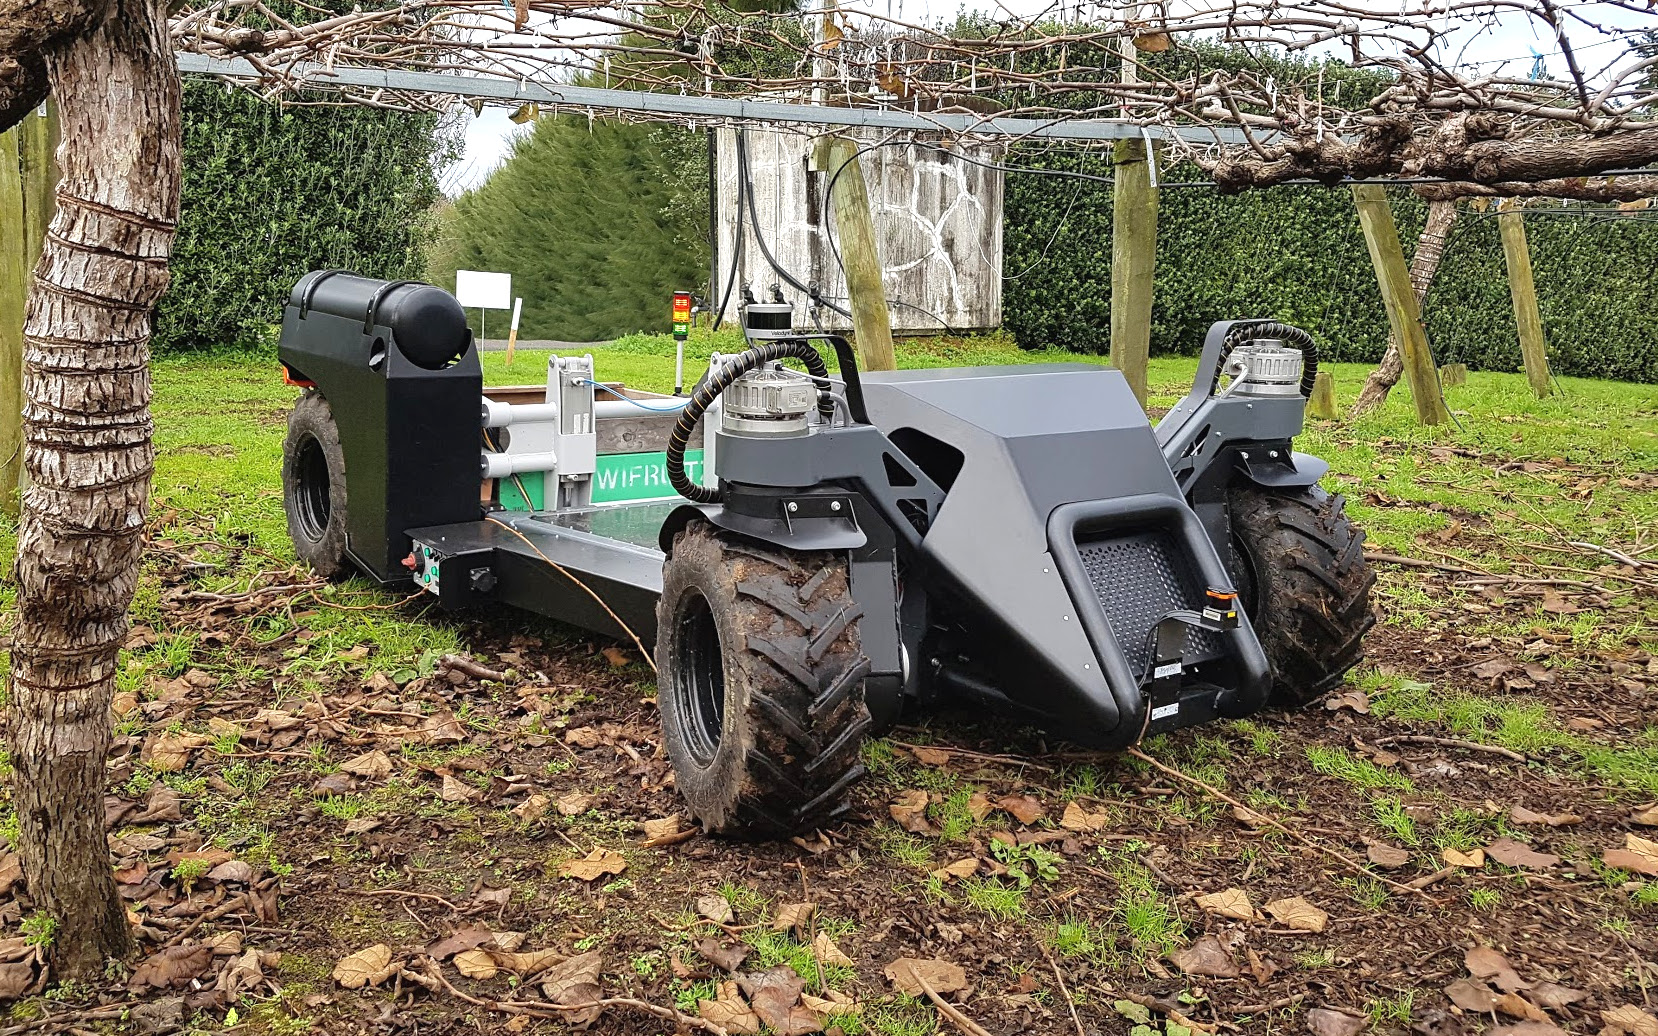
\includegraphics[width=\linewidth]{imgs/photos/suzy_general.jpg}
        \caption{
            Photo of the platform in a kiwifruit orchard.
        }
        \label{fig:suzy}
    \end{figure}

\section{Review}
\label{sect:review}

    The introduction of computers and digital camera technology during the 1980s sparked research into creating autonomous vehicles for agricultural use \cite{Li2009}.
    When publishing details of an autonomous vehicle in 1999, Tillett et~al.\@ cites difficulties dealing with variability in lighting and the environment as the reason no commercial ready vehicles were available at the time.
    The vehicle used wheel encoders, a compass, and accelerometers for odometry information, and featured a camera based row guidance system.
    It was capable of spraying individual plants whilst autonomously driving at \SI{2.5}{\kilo\meter\per\hour}.
    
    In 2002, two autonomous robots designed for weed mapping and control were published \citep{Pedersen2002,Astrand2002}.
    The platforms in these works were relatively simple in terms of their design, referring only to the chassis and drive system, as they are still in a prototype stage.
    Both were Ackermann based and designed for field crops.
    The vehicle presented by \cite{Pedersen2002} was designed to follow pre-defined paths through row-crops, but the authors found that this was impractical without a dedicated row guidance sensor.
    They then discuss a revision of their prototype that features a four wheel steering and drive system and integrating both GPS and a row guidance measurements.
    This work demonstrates a need to combine data from multiple sensor types, which becomes the standard henceforth.
    Mention at this time was made of utilising a Controller Area Network (CAN) to communicate with drive and steering modules on the revised unit due to it being a dominating standard in agricultural vehicles.
    \colorbox{yellow}{Did this next prototype ever get published?}
    
    
    \cite{Bak2004} present a relatively advanced robotic platform based on a four wheel steering geometry.
    The authors noted that the control strategy for the four independently controlled wheels was non-trivial.
    Like the platform presented earlier by Pederson et~al.\@, it combined a compass, gyroscope and GPS for odommetry.
    However, it also featured encoder feedback, a row detection sensor and a GPS unit utilising Real Time Kinematic (RTK) corrections from a base station.
    RTK-GPS is capable of providing positioning with accuracies of around \SI{2}{\centi\meter}.
    Their robot utilised a CAN bus for some aspects of system communication.

    In 2008, Klose et~al.\@ publish details of `Weedy', a autonomous weed control robot for field use.
    It used a simplistic four wheel steering geometry.
    There are few details on the sensor selection apart from mention of the use of cameras and 'acoustic distance sensors'.
    Presumably the selection of drive geometry on this robot is a cost/complexity optimisation.
    It too makes use of a CAN bus for communication between on-board modules.

    The following year, many the same authors appearing on the `Weedy' paper published details an autonomous robotic platform with four wheel steering named BoniRob \citep{Ruckelshausen2009}.
    BoniRob had the ability raise and lower itself and alter its wheel placement by actuating the arms to which the motors are attached to.
    Similar to the unit presented by Bak et~al.\@ it features a gyroscope and RTK-GPS for localisation.
    It introduces the use of both 2D and 3D laser-scanning (or lidar) for perception and row detection.
    A CAN bus is used to control the low level systems (such as the drive control) and ethernet connections for higher level communication.
    The authors created a simulated model of the platform using Gazebo in which they could test the many-degrees-of-freedom drive system.

    Of particular relevance is the work of Scarfe et~al.\@ on an autonomous kiwifruit picking robot \citep{scarfe2009, Scarfe2012}.
    That work involved the creation of a hydraulically driven platform with Ackermann steering to which four fruit harvesting arms were integrated.
    For navigation it used lidar, camera based machine vision, GPS, and a compass.
    The development of that robot forms much of the foundation for the work presented here.

    Common among these vehicles is the use of sensor fusion, whereby data from multiple sensors is merged and filtered.
    This provides a way to combine the advantages of multiple sensor types, and the benefit of redundancy from multiple sensors, into a single computation space.
    With regards to the use of RTK-GPS of perception based guidance systems, Slaughter et~al.\@ points out the trade-off of requiring an ``unobstructed ``view'' of the sky from all parts of the field'' \citep{Slaughter2008}.
    Additionally, multi-path signal propagation caused by nearby foliage or the geometry of the land itself presents its own mode of failure \citep{Durrant-Whyte2005}.
    This requirement can not be satisfied under the canopy of a kiwifruit orchard which are usually surrounded by tall wind-breaking hedges.
    A separate feasibility analysis highlighted the use of RTK-GPS systems as a significant cost in yearly subscriptions alone \citep{Pedersen2006}.
    Torii suggests a combination of both RTK-GPS and machine vision systems to be the most promising system going forward based on reductions in costs and increases in performance of these systems \cite{Torii2000}.
    While \cite{Li2009} concludes that either GPS and machine vision, or GPS and lidar will be used together as a development trend.

    This review has focused on the automation of vehicles specifically designed for autonomous driving in agriculture.
    Much of the sensing requirements discussed for autonomous navigation have been developed on existing vehicles converted for computer control.
    Most, if not all, sensing and navigation developments made on those vehicle also apply here.

    % Of the reported platforms designed specifically to be autonomous there appears to be an equal split between Ackermann and four-wheel steering geometries.
    % The ability of four wheel steering to pivot about the centre of the vehicle, as opposed to the centre of the rear wheels with an Ackermann geometry, offers little gain in an orchard environment.
    % Not only can Ackermann geometry offer a reduction in mechanical complexity, but also removes the need to develop the ``non-trivial'' control strategies.

    \cite{Blackmore2007} envisaged significant reductions in production costs by re-purposing parts already in use in the agricultural and automotive industry.
    While not a physical component, the CAN is one such technology borrowed from the automotive industry aiding developmental of low-level communications.
    Many of the platforms reviewed, especially the more recent ones, made use of this protocol for real-time communication.
    Platforms designed for open field crops appear to favor four-wheel steering over the more traditional Ackermann geometry.
    The use of simulation tools allowed the creators of BoniRob to develop and test their mobility system separate of the physical hardware.

    \color{red}
        shift focus here to the mechanical aspects, but keep whatever ties in with what Jamie has done in terms of sensor selection
    \color{black}

\section{Mechanical design}
\label{sect:mechanical}

    \begin{figure}[htb]
        \centering
        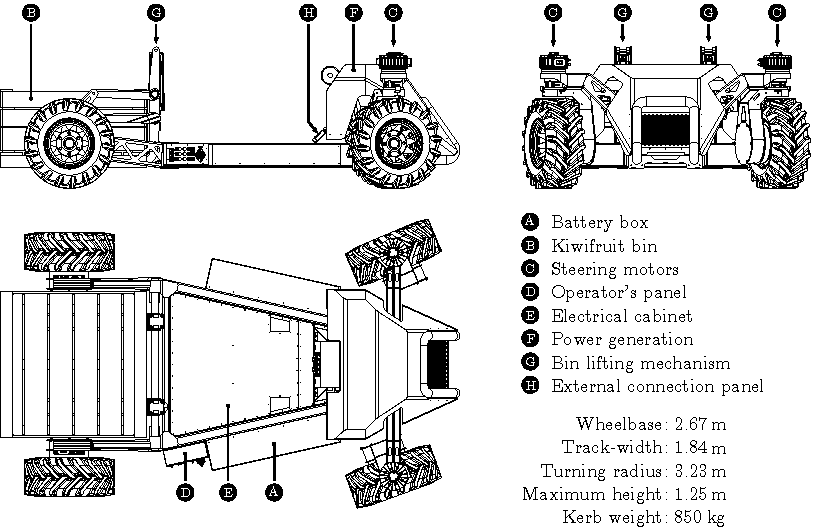
\includegraphics[width=\linewidth]{imgs/profile_views/AMMP-All-Labelled.pdf}
        \caption{Profile drawings of the robotic platform with kiwifruit bin.}
        \label{fig:AMMP}
    \end{figure}

    Canopy heights of kiwifruit orchards range between \SI{1300}{\milli\meter} and \SI{1700}{\milli\meter}.
    Modules on the platform need additional clearance from the canopy in addition the height of the module itself.
    To maximise space available to the modules it carries, the platform must be low-slung where these modules attach.
    Figure \ref{fig:AMMP} illustrates the design; area for mounting modules is visible between markers `F' and `E' in the side view (top left).

    Steering geometry is Ackermann based with independent motors on the front wheels for actuation.
    The ability to actuate the angles individually simplifies the mechanical geometry needed to coordinate steering, particularly at extreme steering angles.
    Each steering wheel has the freedom to rotate \SI{340}{\degree}, providing the ability to pivot about the centre of its rear wheels.
    This sets the turning circle to be twice the distance from the centre of the rear wheels to the front of the vehicle.
    Implementing four wheel steering would allow the centre of rotation to move to the centre of the vehicle, decreasing the turning circle to the total length of the vehicle.
    As the headlands of kiwifruit orchards are sized for tractors to turn between rows, Ackermann based steering is sufficient.
    The implementation of Ackermann geometry simplifies the overall design and increases the usable area at the rear of the vehicle; allowing a full-size kiwifruit bin and lifting mechanism to occupy this space.
    Not only does it offer a reduction in mechanical complexity, but removes the need to develop ``non-trivial'' control strategies.
    A differential drive, or skid steer, system was expected to cause ground damage to a level considered unacceptable to orchard owners.

    The platform has no suspension, other than its tries, and features a front pivoting axle to maintain three points of contact with the ground.
    Each wheel is mounted directly to a 40:1 fixed ratio planetary gear gearbox connected to a permanent magnet, brushless AC motor.
    The gearbox-motor combination allows the platform to travel at a maximum speed of \SI{10}{\kilo\meter\per\hour}.
    In total, the drive system is capable of delivering \SI{25.6}{\kilo\watt} of power and \SI{3.3}{\kilo\newton\meter} of torque continuously.
    With these specifications it is capable of accelerating from a stand-still to its maximum speed at an incline of \SI{20}{\degree} carrying a \SI{600}{\kilo\gram} payload in \SI{2.0}{\second}.

    At the front of the platform sits a power generation unit including a petrol engine, air compressor, and alternator.
    These are connected together by a single timing belt.
    The compressor and alternator are activated electronically by a custom power generation controller.
    Fuel and compressed air tanks sits over the right-hand rear wheel, which are visible in figure \ref{fig:suzy}.
    Battery modules attached to the sides of the chassis each house fifteen lithium-iron-phosphate batteries.

    Unloaded, the machine has an estimated mass of \SI{850}{\kilo\gram}, including the power generation unit.
    It has been designed and tested to be capable of carrying \SI{1000}{\kilo\gram} in it's payload space.
    With that load, the platform's maneuverability and ability to brake or accelerate was not noticeably affected.
    \colorbox{yellow}{Stuff starts getting flaky from here.}

\section{System Architecture}
\label{sect:hardware}

    \begin{figure}[htb]
        \centering
        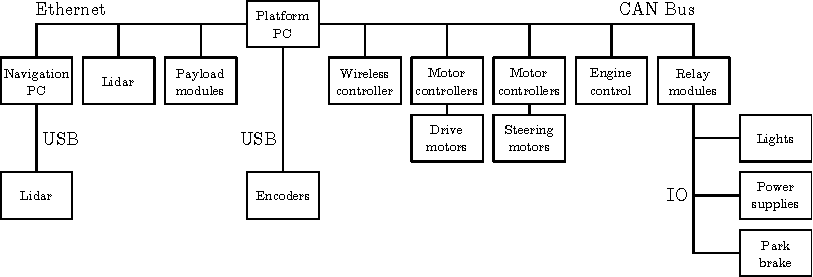
\includegraphics[width=\linewidth]{imgs/system_diagram/diagram_v3.pdf}
        \caption{Hardware level system diagram showing the types of interfaces and relative relations on the platform.}
        \label{fig:system_diagram}
    \end{figure}
    Ethernet, USB, and CAN busses are connect each part of the system as shown in figure \ref{fig:system_diagram}.
    A computer dedicated to processing sensing data related to navigation is connected to the platform's `System PC' via ethernet.
    The open source Robotic Operating System (ROS) is used to facilitate communicate between the two computers.
    Not only is ROS used for inter-computer communication, but also within separate software nodes running on the same machine.
    For example, a node running on the `Driving PC' takes information from a lidar and publishes it on a topic that another node on the same PC has subscribed to.
    The subscribing node then processes the data and generates drive commands which are then published on another topic that the `System PC' is subscribed to.
    From there, the `System PC' will further process that to calculate the steering angles and drive velocities based on the Ackermann geometry and publish it to a node that puts those commands on the CAN bus.

    \colorbox{yellow}{Maybe time for another diagram (software block diagram?)}

    % Include system layout diagram
    Relay modules connected to the main computer via the system's CAN bus give a means of shutting down subsystems.
    They are used to control various outputs on the platform, such as a machine state indicators, electro-actuated park brakes, and the supply of power to sub-systems. 
    Additionally, the relays monitor the platform's CAN bus to ensure that synchronisation messages are being sent out in a timely manner.
    Monitoring the frequency of these messages is one way to determine the state of the computer generating them, which in this case it is the system PC.
    In the event that the synchonisation messages begin to vary in frequency, or stop, the relays cut power to all subsystems and engage the brakes.

    % A wireless safety-rated controller is used to remotely control platform.
    % The controller 
    % The controller provides the operator with a way of entering the platform into autonomous mode, manual control, triggering an emergency stop, or enabling/disabling auxiliary systems.

\section{Software}
\label{sect:software}
    \color{red}
        OLD CONTENT: Unsure about what to put in this section. Jamie, you are free to completely hijack this.
    \color{black}
    The control software is comprised of individual nodes, writen in either C++ or Python, linked together using Robot Operating System (ROS) for interprocess communication.
    The system runs on Ubuntu Server 16.04 on an Intel NUC, a compact x86 based PC.
    A model of the robot platform has been depeloped for use with Gazebo simulation software.
    Such a model provides a way to test steering and movement strategies before deploying them on the hardware.

\section{Sensor selection}
\label{sect:sensors}
    [Jamie's section]

\section{Autonomous Driving}
\label{sect:autonomous}
    \color{red}
        It would be great if we could put something in here with regards to how well the platform navigates an orchard.
        If you don't want to write it, I can write something generic and put it in for you to approve.
        Alternatively, you may not want anything in here relating to the navigation performance.
    \color{black}
    \begin{figure}[htb]
        \centering
        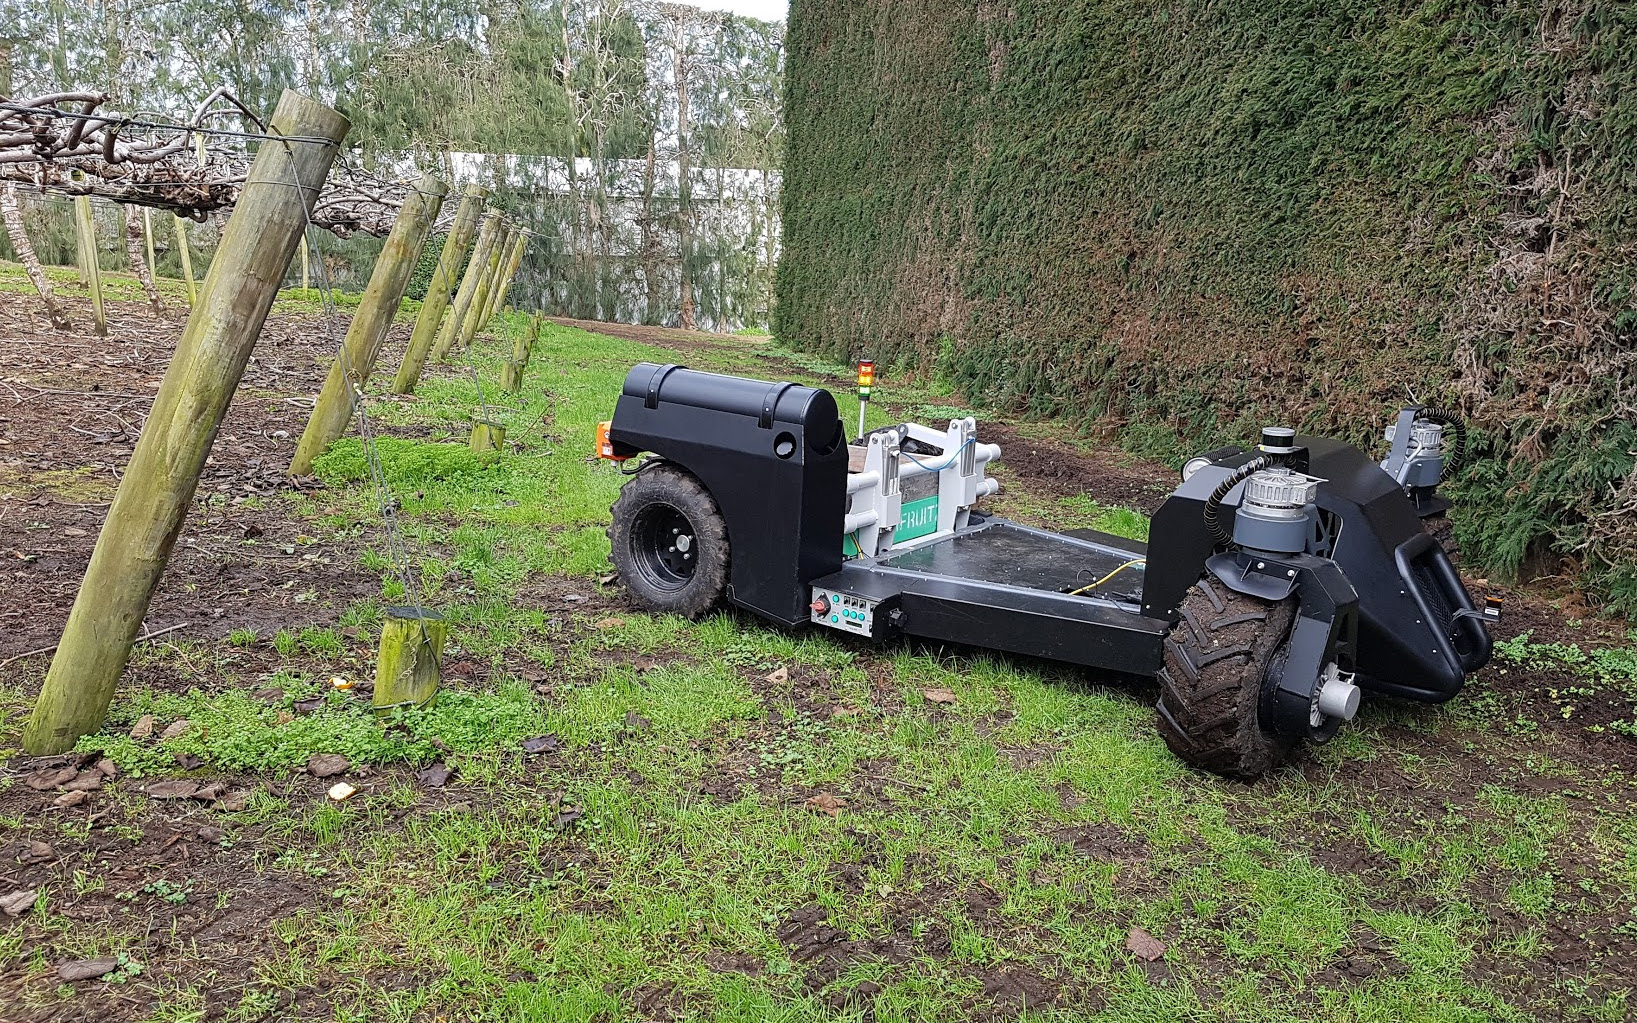
\includegraphics[width=\linewidth]{imgs/photos/suzy_turning.jpg}
        \caption{
            Photo showing the platform performing a row-end turn
        }
        \label{fig:suzy_turning}
    \end{figure}

\section{Discussion}
    TODO: Generally summerise the platform, its ability to carry stuff, suitability for the orchard environment, and its ability to drive autonomously.

\section*{Acknowledgements}
This research was funded in-part by a grant from the New Zealand Ministry of Business Innovation and Employment.
The authors acknowledge contributions from Phillip Ross and Gordon Neshausen in the design and fabrication of the platform.

\section{Jamie-Mark communication}
You are free to suggest anything about anything.
Maybe you want to add someone to the authors list?
Maybe you don't like the focus of the review, or think a review is not necessary.
Perhaps you can think of something that would go well in the paper that I've not mentioned.

% Diagram of sensor placement
% Lidar units and visibility
% All electric drive system based on ackermann steering
% Sevcons modified to allow for direct CAN control.
% Power system and battery pack
% power-gen capable of charging battery pack approx 24hour duty
% Drive motors used as steering motors
% Control based on ROS, complete with gazebo simulation
% State the turning circle.
% State the mass and payload capability
% Show the area for drop-on modules (diagram)
% Integrated bin lifting mechanism
% Platform electronics

% Sections:
%   Mechanical design
%   Hardware and sensors
%   Software architecture


%% The Appendices part is started with the command \appendix;
%% appendix sections are then done as normal sections
%% \appendix

%% \section{}
%% \label{}

%% References
%%
%% Following citation commands can be used in the body text:
%%
%%  \citet{key}  ==>>  Jones et al. (1990)
%%  \citep{key}  ==>>  (Jones et al., 1990)
%%
%% Multiple citations as normal:
%% \citep{key1,key2}         ==>> (Jones et al., 1990; Smith, 1989)
%%                            or  (Jones et al., 1990, 1991)
%%                            or  (Jones et al., 1990a,b)
%% \cite{key} is the equivalent of \citet{key} in author-year mode
%%
%% Full author lists may be forced with \citet* or \citep*, e.g.
%%   \citep*{key}            ==>> (Jones, Baker, and Williams, 1990)
%%
%% Optional notes as:
%%   \citep[chap. 2]{key}    ==>> (Jones et al., 1990, chap. 2)
%%   \citep[e.g.,][]{key}    ==>> (e.g., Jones et al., 1990)
%%   \citep[see][pg. 34]{key}==>> (see Jones et al., 1990, pg. 34)
%%  (Note: in standard LaTeX, only one note is allowed, after the ref.
%%   Here, one note is like the standard, two make pre- and post-notes.)
%%
%%   \citealt{key}          ==>> Jones et al. 1990
%%   \citealt*{key}         ==>> Jones, Baker, and Williams 1990
%%   \citealp{key}          ==>> Jones et al., 1990
%%   \citealp*{key}         ==>> Jones, Baker, and Williams, 1990
%%
%% Additional citation possibilities
%%   \citeauthor{key}       ==>> Jones et al.
%%   \citeauthor*{key}      ==>> Jones, Baker, and Williams
%%   \citeyear{key}         ==>> 1990
%%   \citeyearpar{key}      ==>> (1990)
%%   \citetext{priv. comm.} ==>> (priv. comm.)
%%   \citenum{key}          ==>> 11 [non-superscripted]
%% Note: full author lists depends on whether the bib style supports them;
%%       if not, the abbreviated list is printed even when full requested.
%%
%% For names like della Robbia at the start of a sentence, use
%%   \Citet{dRob98}         ==>> Della Robbia (1998)
%%   \Citep{dRob98}         ==>> (Della Robbia, 1998)
%%   \Citeauthor{dRob98}    ==>> Della Robbia


%% References with bibTeX database:

\bibliographystyle{model5-names}
\bibliography{library}

%% Authors are advised to submit their bibtex database files. They are
%% requested to list a bibtex style file in the manuscript if they do
%% not want to use model5-names.bst.

%% References without bibTeX database:

% \begin{thebibliography}{00}

%% \bibitem must have one of the following forms:
%%   \bibitem[Jones et al.(1990)]{key}...
%%   \bibitem[Jones et al.(1990)Jones, Baker, and Williams]{key}...
%%   \bibitem[Jones et al., 1990]{key}...
%%   \bibitem[\protect\citeauthoryear{Jones, Baker, and Williams}{Jones
%%       et al.}{1990}]{key}...
%%   \bibitem[\protect\citeauthoryear{Jones et al.}{1990}]{key}...
%%   \bibitem[\protect\astroncite{Jones et al.}{1990}]{key}...
%%   \bibitem[\protect\citename{Jones et al., }1990]{key}...
%%   \harvarditem[Jones et al.]{Jones, Baker, and Williams}{1990}{key}...
%%

% \bibitem[ ()]{}

% \end{thebibliography}

\end{document}

%%
%% End of file `elsarticle-template-5-harv.tex'.
